%!TEX root=paper/thesis.tex
\subsection{Features of the state}\label{sec:det_features}

\PM{Open vs Closed Loop}
An \emph{open-loop} policy, such as the common classifier cascade \cite{Viola2004}, takes actions in a sequence that does not depend on observations received from previous actions.
In contrast, our goal is to learn a dynamic, or \emph{closed-loop}, policy, which would exploit the signal in scene and inter-object context for a maximally efficient path through the actions.

\PM{State}
We refer to the information available to the decision process as the \emph{state} $s$.
The state includes the current estimate of the distribution over class presence variables $P(\mathbf{C}) = \{P(C_0), \ldots, P(C_K)\}$, where we write $P(C_k)$ to mean $P(C_k=1)$ (class $k$ is present in the image).
Additionally, the state records that an action $a_i$ has been taken by adding it to the initially empty set $\mathcal{O}$ and recording the resulting observations $o_i$.
We refer to the current set of observations as $\mathbf{o} = \{o_i | a_i \in \mathcal{O}\}$.
The state also keeps track of the time into episode $t$, and the setup and deadline times $T_s,T_d$.

\PM{Dynamic features}
Our policy is at its base determined by a linear function of the features of the state:
\begin{align}
\pi(s) = \argmax_{a_i \in \mathcal{A} \setminus \mathcal{O}} \theta_\pi^\top \phi(s,a_i).
\end{align}
Since we want to be able to learn a dynamic policy, the observations $\mathbf{o}$ that are part of the state $s$ should play a role in determining the value of a potential action.

We include the following quantities as features $\phi(s,a)$:

\begin{tabularx}{0.8\linewidth}{p{0.23\linewidth}p{0.69\linewidth}}
$P(C_a)$ & The prior probability of the class that corresponds to the detector of action $a$ (omitted for the scene-context action).\\
$P(C_0|\mathbf{o}) \ldots P(C_K|\mathbf{o})$ & The probabilities for all classes, conditioned on the current set of observations.\\
$H(C_0|\mathbf{o}) \ldots H(C_K|\mathbf{o})$ & The entropies for all classes, conditioned on the current set of observations. \\
\end{tabularx}

Additionally, we include the mean and maximum of $[H(C_0|\mathbf{o}) \ldots H(C_K|\mathbf{o})]$, and $4$ time features that represent the times until start and deadline, for a total of $F = 1+2K+6$ features.

\PM{Augmented MDP}
We note that this setup is commonly used to solve Markov Decision Processes \cite{Sutton1998}.
There are two related limitations of MDPs when it comes to most systems of interesting complexity, however: the state has to be functionally approximated instead of exhaustively enumerated; and some aspects of the state are not observed, making the problem a Partially Observed MDP (POMDP), for which exact solution methods are intractable for all but rather small problems \cite{Roy2002}.
Our initial solution to the problem of partial observability is to include features corresponding to our level of uncertainty into the feature representation, as in the technique of \emph{augmented} MDPs \cite{Kwok2004}.

\begin{figure}[h!]
\centering
\begin{subfigure}[t]{.8\linewidth}
    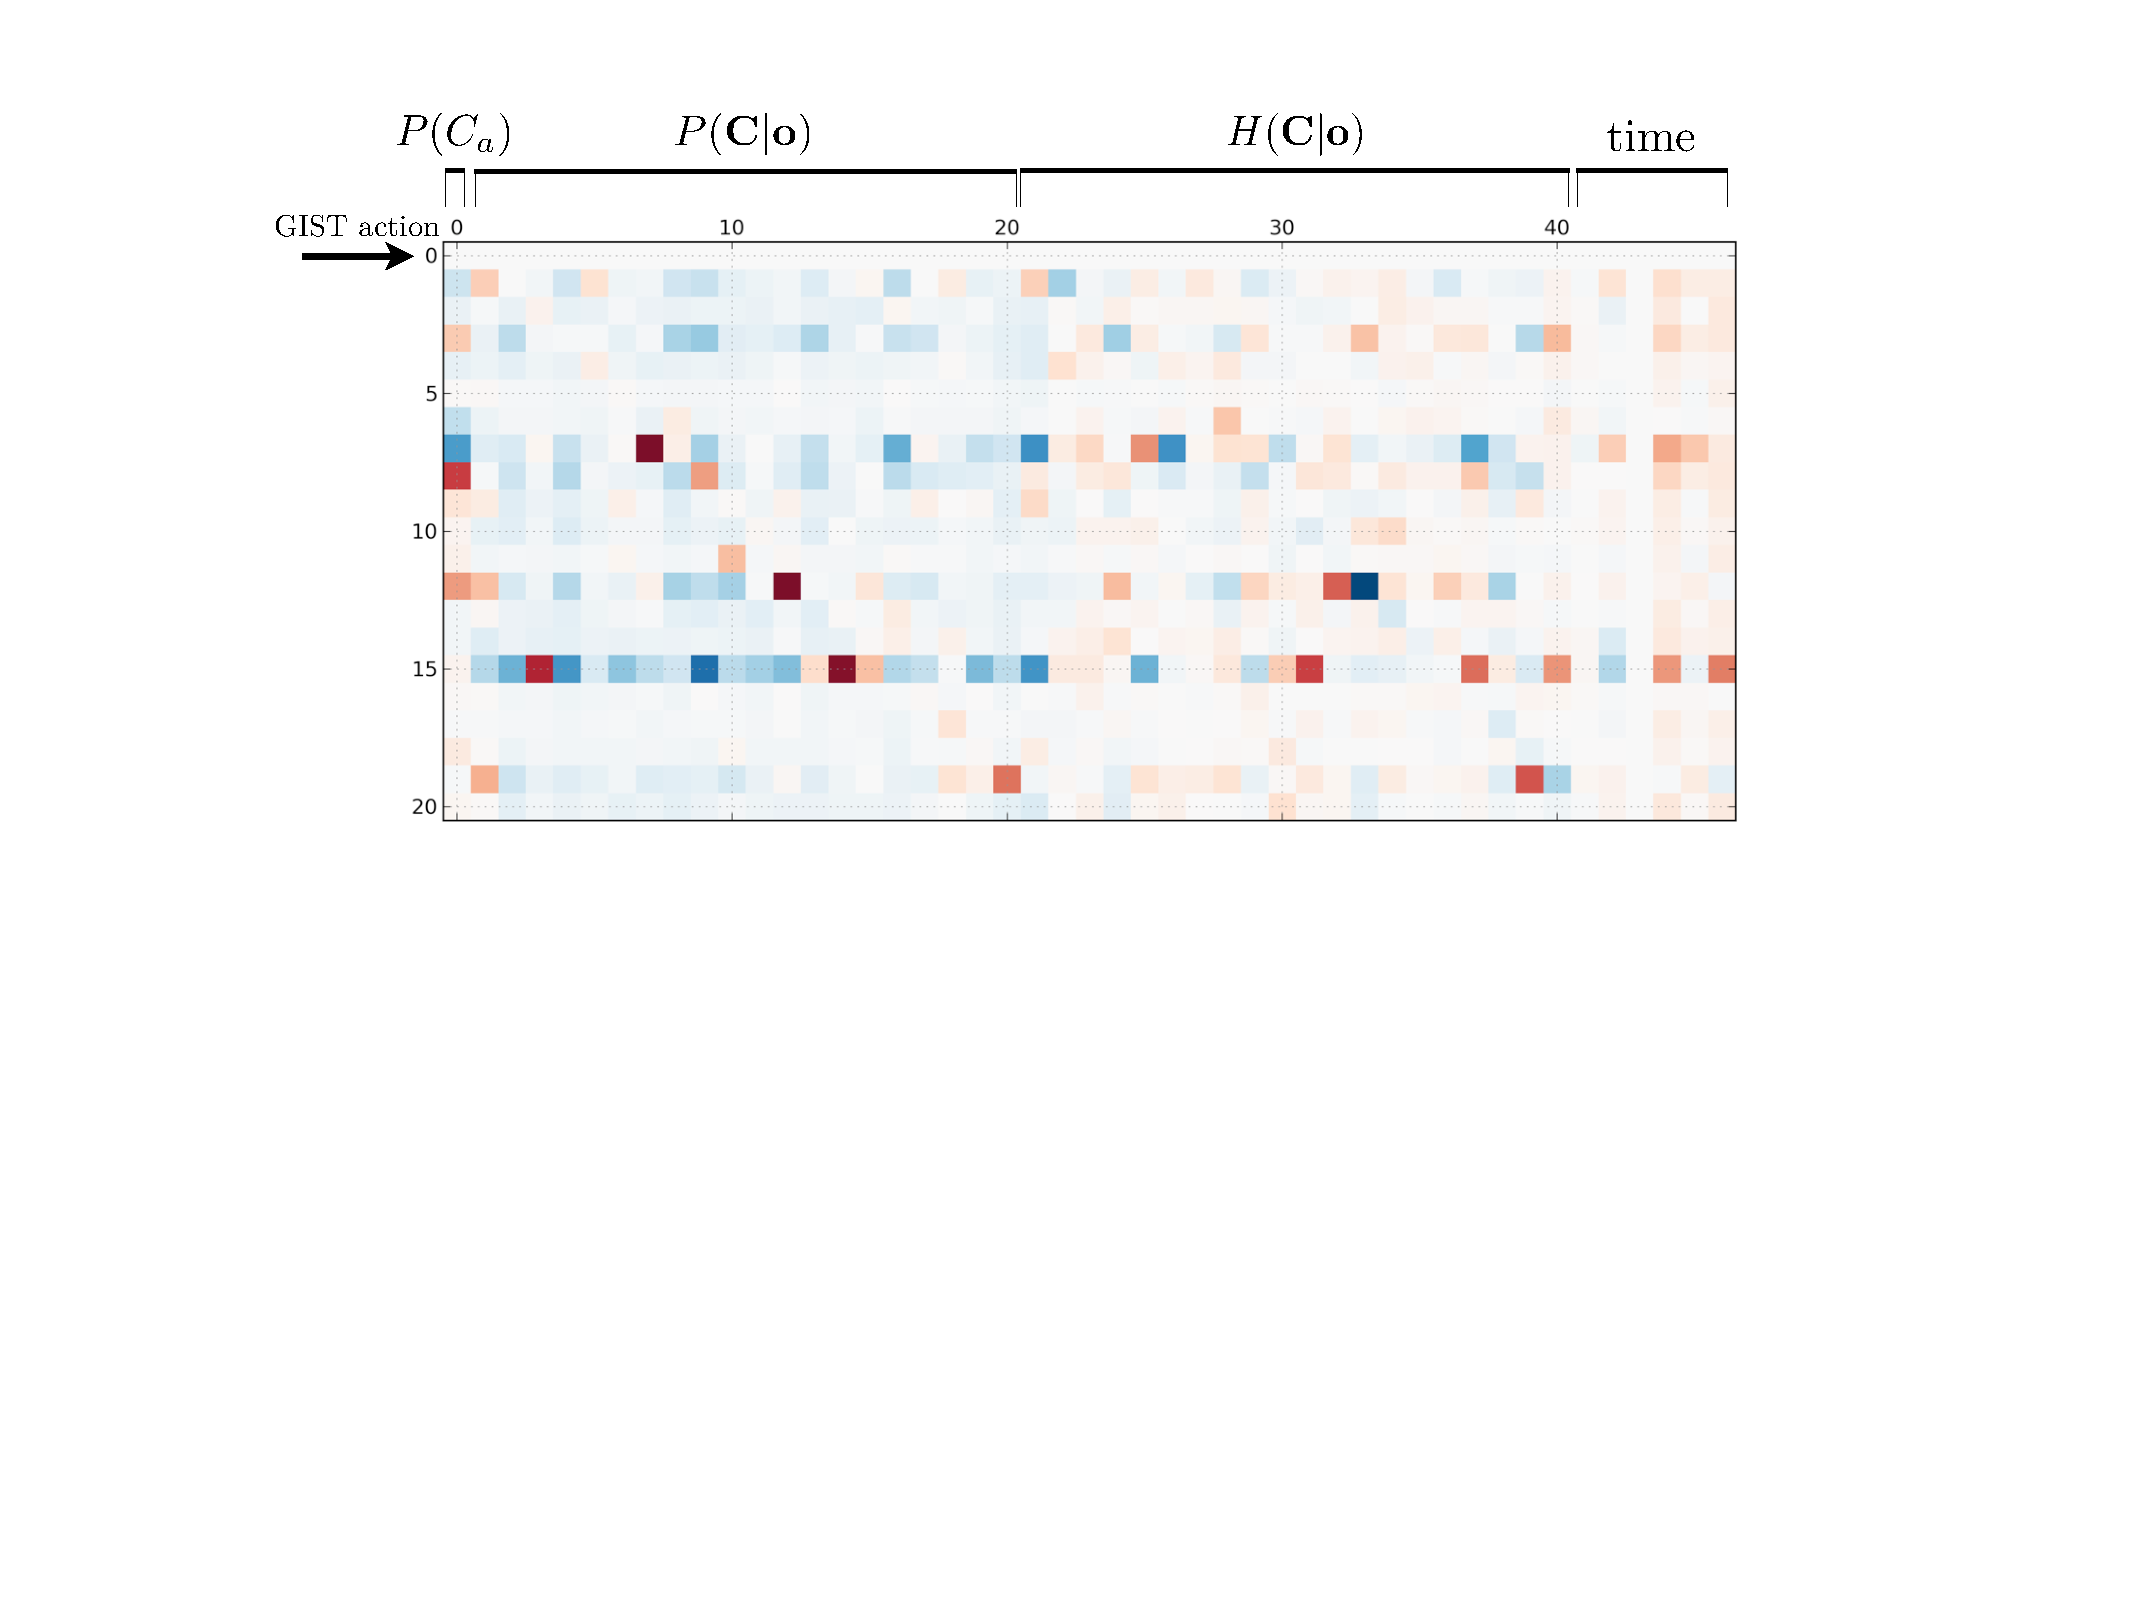
\includegraphics[width=\linewidth]{../../../2011-2012/figures/weights_greedy}
    \caption{Greedy}
\end{subfigure}\\
\begin{subfigure}[t]{.8\linewidth}
    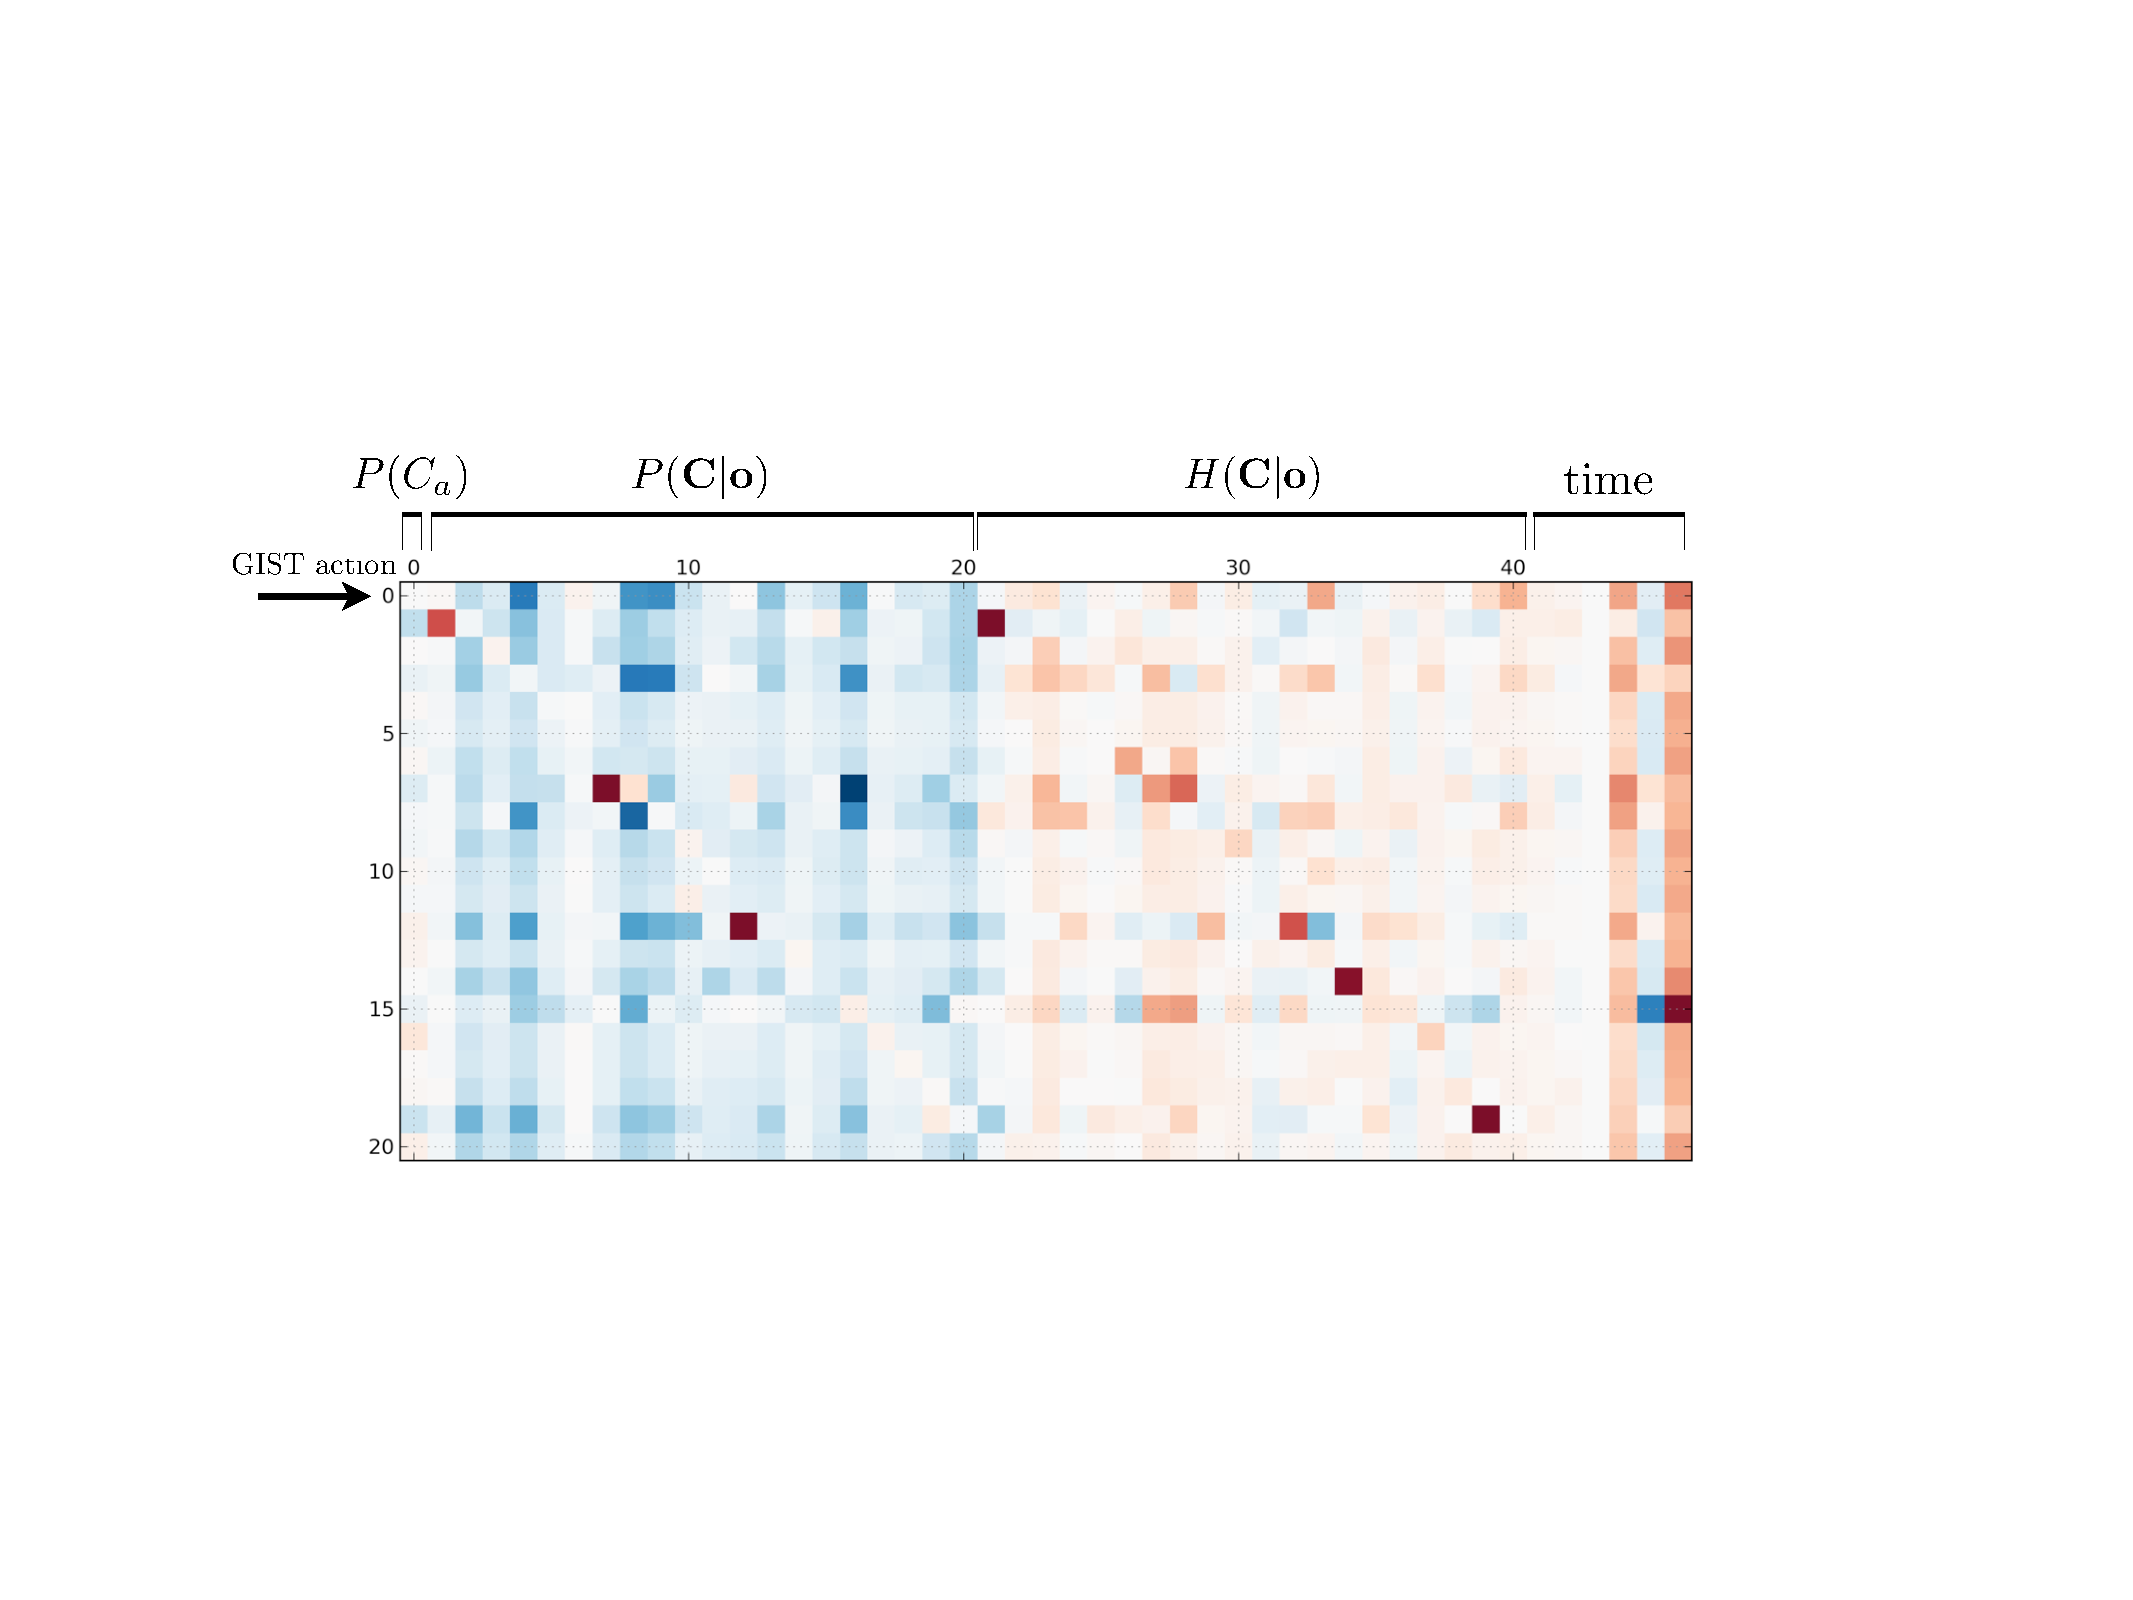
\includegraphics[width=\linewidth]{../../../2011-2012/figures/weights_rl}
    \caption{Reinforcement Learning}
\end{subfigure}
\caption[Learned policy weights for the detection approach.]{
Learned policy weights $\theta_\pi$ (best viewed in color: red corresponds to positive, blue to negative values).
The first row corresponds to the scene-level action, which does not generate detections itself but only helps reduce uncertainty about the contents of the image.
Note that in the greedy learning case, this action is learned to never be taken, but it is shown to be useful in the reinforcement learning case.
}
\label{fig:det_weights}
\end{figure}


\PM{Illustration}
As an illustration, we visualize the learned weights on these features in \autoref{fig:det_weights}, reshaped such that each row shows the weights learned for an action, with the top row representing the scene context action and then next $20$ rows corresponding to the PASCAL VOC class detector actions.
\todo{say something about this}

\subsubsection{Updating with observations}\label{sec:updating}

\PM{Class correlations}
The bulk of our feature representation is formed by probability of individual class occurrence, conditioned on the observations so far: $P(C_0|\mathbf{o}) \ldots P(C_K|\mathbf{o})$.
This allows the action-value function to learn correlations between presence of different classes, and so the policy can look for the most probable classes given the observations.
However, higher-order co-occurrences are not well represented in this form.
Additionally, updating $P(C_i|\mathbf{o})$ presents choices regarding independence assumptions between the classes.

\PM{Direct vs. MRF update}
We evaluate two approaches for updating probabilities: \emph{direct} and \emph{MRF}.
In the \emph{direct} method, $P(C_i|\mathbf{o}) = score(C_i)$ if $\mathbf{o}$ includes the observations for class $C_i$ and $P(C_i|\mathbf{o}) = P(C_i)$ otherwise.
This means that an observation of class $i$ does not directly influence the estimated probability of any class but $C_i$.
The \emph{MRF} approach employs a pairwise fully-connected Markov Random Field (MRF), as shown in Figure~\ref{fig:figure1}, with the observation nodes set to $score(C_i)$ appropriately, or considered unobserved.

\PM{Learning MRF}
The graphical model structure is set as fully-connected, but some classes almost never co-occurr in our dataset.
Accordingly, the edge weights are learned with $L_1$ regularization, which obtains a sparse structure \cite{Lee2006}.
All parameters of the model are trained on fully-observed data, and Loopy Belief Propagation inference is implemented with an open-source graphical model package \cite{Jaimovich2010}.

\PM{Details}
An implementation detail: $score(C_i)$ for $a_{{det}_i}$ is obtained by training a probabilistic classifier on the list of detections, featurized by the top few confidence scores and the total number of detections.
Similarly, $score(C_i)$ for $a_{gist}$ is obtained by training probabilistic classifiers on the GIST feature, for all classes.
